\documentclass[11pt]{article}
\usepackage[a4paper,margin=0.85in]{geometry}
\usepackage{tikz}
\usetikzlibrary{arrows.meta,positioning,shapes.geometric}
\usepackage{pgfplots}
\pgfplotsset{compat=1.18}
\usepackage{booktabs}
\usepackage{xcolor}
\usepackage{enumitem}
\usepackage[hidelinks]{hyperref}
\usepackage{titlesec}

% viewer palette
\definecolor{scaf}{HTML}{2F9E6E}
\definecolor{epi}{HTML}{C0392B}
\definecolor{ab}{HTML}{2B47D6}
\definecolor{nat}{HTML}{707A86}
\definecolor{ink}{HTML}{1A1A1A}
\definecolor{accent}{HTML}{1B4A86}
\definecolor{pale}{HTML}{EEF3F9}

\titleformat{\section}{\large\bfseries\color{accent}}{}{0pt}{}
\titlespacing{\section}{0pt}{10pt}{3pt}
\setlist[itemize]{leftmargin=1.3em,itemsep=1pt,topsep=2pt}
\pagestyle{empty}
\setlength{\parindent}{0pt}
\setlength{\parskip}{3pt}

\begin{document}

{\LARGE\bfseries episcaf --- RFD4 scaffolding engine}\\[2pt]
{\color{ink}\large Status spec}\hfill{\color{ink}2026-11-25 \;\textbf{\textbullet}\; branch \texttt{rfd4-engine}}\\[-4pt]
\rule{\linewidth}{0.8pt}

\vspace{2pt}
A lab-facing web tool: upload an antigen, pick an epitope, click submit. A GPU campaign runs on the
lab's Gemini cluster and returns protein-scaffold designs ranked by a composite score, each with a
per-design 3D viewer. The engine is John Altin's RFD4 pipeline ported to Python.

\vspace{-2pt}
\section*{Pipeline}
\vspace{2pt}
\begin{center}
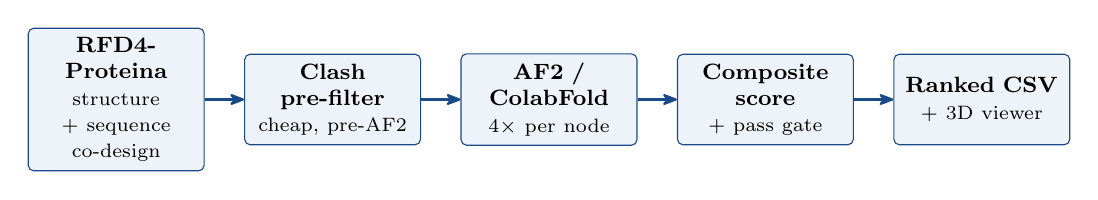
\begin{tikzpicture}[>={Stealth[round]},node distance=0.5cm,
  pb/.style={draw,rounded corners=2pt,fill=pale,draw=accent,minimum height=1.15cm,
             text width=2.0cm,align=center,font=\footnotesize}]
\node[pb](a){\textbf{RFD4-Proteina}\\\scriptsize structure + sequence co-design};
\node[pb,right=of a](b){\textbf{Clash}\\\textbf{pre-filter}\\\scriptsize cheap, pre-AF2};
\node[pb,right=of b](c){\textbf{AF2 / ColabFold}\\\scriptsize 4$\times$ per node};
\node[pb,right=of c](d){\textbf{Composite}\\\textbf{score}\\\scriptsize + pass gate};
\node[pb,right=of d](e){\textbf{Ranked CSV}\\\scriptsize + 3D viewer};
\draw[->,accent,thick](a)--(b); \draw[->,accent,thick](b)--(c);
\draw[->,accent,thick](c)--(d); \draw[->,accent,thick](d)--(e);
\end{tikzpicture}
\end{center}
\vspace{-3pt}
{\footnotesize Over-generation is cheap: RFD4 makes up to 128 backbones to find \emph{N} clash-free
ones, so cost scales with \emph{N} (the designs AF2 folds), not with how many are discarded.}

\section*{Inputs and knobs}
\begin{itemize}
  \item \textbf{Two ways to define the epitope:} \emph{antibody contacts} (upload a complex; residues
        within 4\,\AA\ of the bound partner) or \emph{candidate regions} (growPatch on a lone antigen).
  \item \textbf{Number of scaffolds:} user-set, default 32, max 128 --- the number AF2 folds.
  \item \textbf{Design length} 103; multi-chain / high-residue-number epitopes handled via compact input.
\end{itemize}

\section*{Scoring}
The composite is a weighted sum of saturating terms (lower-is-better), plus a pass-gate bonus; a design
passes at composite~$\ge 1.8$. Our composite reproduces John's to the digit on real output.

\begin{center}\footnotesize
\begin{tabular}{@{}lcl@{}}
\toprule
\textbf{Term} & \textbf{Weight} & \textbf{Meaning}\\
\midrule
Antibody clashes & 0.45 & scaffold residues overlapping the Fab (0 required to pass)\\
Epitope RMSD & 0.25 & backbone deviation of the presented epitope\\
Overall RMSD & 0.20 & AF2 model vs.\ the generated design\\
Mean PAE & 0.10 & AF2 predicted aligned error\\
\bottomrule
\end{tabular}
\end{center}
\textbf{No-antibody case:} AOMclash reads a learned antibody-occupancy map ($\sim$3\,ms/design) and its
score replaces the clash count in the 0.45 term, so lone-antigen designs are ranked by accessibility.

\section*{Performance}
First instrumented run: 32 designs on one A100, 86\,min, 1.43 GPU-hr. AF2 is essentially the whole cost
and is independent per design, so we fold 4 at a time on the 4-GPU A100 nodes.

\begin{center}
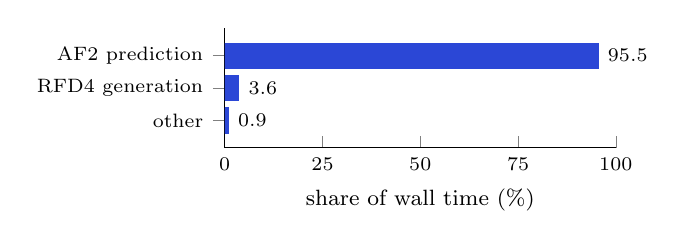
\begin{tikzpicture}
\begin{axis}[
  width=0.54\linewidth,height=3.1cm,xbar,xmin=0,xmax=100,
  bar width=9pt,enlarge y limits=0.42,axis x line*=bottom,axis y line*=none,
  xlabel={\footnotesize share of wall time (\%)},
  xtick={0,25,50,75,100},
  ytick=data,yticklabels={AF2 prediction,RFD4 generation,other},
  y tick label style={font=\scriptsize},x tick label style={font=\scriptsize},
  nodes near coords,every node near coord/.append style={font=\scriptsize},
  nodes near coords style={/pgf/number format/fixed,/pgf/number format/precision=1},
]
\addplot[fill=ab,draw=ab] coordinates {(95.5,2) (3.6,1) (0.9,0)};
\end{axis}
\end{tikzpicture}
\hspace{0.03\linewidth}
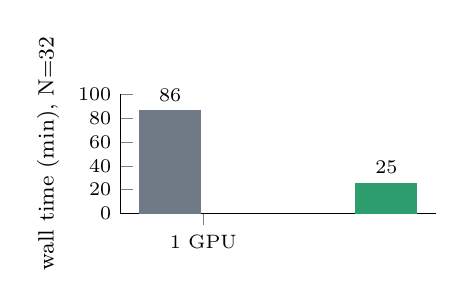
\begin{tikzpicture}
\begin{axis}[
  width=0.46\linewidth,height=3.1cm,ybar,ymin=0,ymax=100,
  bar width=22pt,enlarge x limits=0.55,axis y line*=left,axis x line*=bottom,
  ylabel={\footnotesize wall time (min), N=32},
  symbolic x coords={1 GPU,4 GPUs},xtick=data,
  x tick label style={font=\scriptsize},y tick label style={font=\scriptsize},
  nodes near coords,every node near coord/.append style={font=\scriptsize},
]
\addplot[fill=nat,draw=nat] coordinates {(1 GPU,86)};
\addplot[fill=scaf,draw=scaf] coordinates {(4 GPUs,25)};
\end{axis}
\end{tikzpicture}
\end{center}
\vspace{-4pt}
{\footnotesize Per-task cost for budgeting: AF2 $\approx$0.043 GPU-hr/design; generation
$\approx$0.05 GPU-hr/run (flat). 4$\times$ folding: $\sim$25\,min typical, $\sim$35\,min with a
slow-MSA design. v100 nodes are a lower-contention option since the folds are short.}

\section*{Per-design viewer}
Click a design in the results table and its structure docks on the right:
{\color{scaf}\textbf{scaffold}}, {\color{epi}\textbf{epitope}},
{\color{nat}\textbf{native antigen}}, {\color{ab}\textbf{antibody}}, and steric clashes, with
layer toggles, pan, spin, and an antibody-occupancy mesh. The epitope aligns onto the native frame, so
the viewer's epitope RMSD matches the scored value.

\section*{Status}
\textbf{Live now:} both epitope avenues; click-to-submit on Gemini; the scaffold-count knob; 4$\times$
folding; compact input; antibody auto-detection; AOMclash accessibility; the per-design viewer;
step-aware run status; composite-ranked results with downloads.

\textbf{Next:} seeded partial-diffusion rounds (adaptive multi-round --- the biggest quality lever for
hard epitopes; decision logic is in place, child generation is the remaining piece); cross-node scaling
beyond 4 GPUs if large batches need it; the real occupancy-shell mesh in the viewer.

\vspace{4pt}
\rule{\linewidth}{0.4pt}
{\footnotesize Runs on Gemini (RFD4-Proteina + ColabFold on \texttt{gpu-a100}); the web UI + request
broker on Cloud Run; a data-mover worker auto-submits each job. PI: John Altin.}

\end{document}
